% !TeX root=main.tex
% دستور زیر باید در اولین فصل شما باشد. آن را حذف نکنید!
\pagenumbering{arabic}

\chapter{مقدمه} \label{ch:intro}
\thispagestyle{empty}


\section{شرح مسأله} \label{sec:sharh}
\paragraph{}
{
    یکی از مسائلی که امروزه در زمینه کنترل و پایش دستگاه‌های اینترنت اشیاء وجود دارد، عدم یکپارچگی و هماهنگی
    میان دستگاه‌های مختلف است. این دستگاه‌ها از فناوری‌ها، پروتکل‌ها و استانداردهای متنوعی برای ارتباط و عملکرد
    استفاده میکنند، که این تنوع باعث پیچیدگی و مشکلاتی در کنترل و پایش مرکزی آنها میشود. به عنوان مثال، در یک
    بستر اینترنت اشیاء ممکن است دستگاههایی با پروتکلهای ارتباطی مختلف، مانند
    HTTP\footnote{\lr{Hypertext Transfer Protocol}}،
    MQTT\footnote{\lr{Message Queuing Telemetry Transport}}
    و CoAP\footnote{\lr{Constrained Application Protocol}}
    داشته باشند که هر کدام نیازمند روش‌ها و فناوری‌های جداگانه برای کنترل و پایش خود هستند. همچنین، دستگاه‌های
    اینترنت اشیاء ممکن است از نظر تکنولوژی و نوع عملکرد با هم تفاوت داشته باشند. برای مثال، یک سنسور دما و یک قفل هوشمند
    دارای نیازهای کنترل و پایش متفاوتی هستند. این تنوع در دستگاه‌ها باعث پیچیدگی در توسعه و اجرای یک سیستم
    کنترل یکپارچه می‌شود.
    محدودیت منابع نیز یک چالش اساسی در محیط‌های اینترنت اشیاء است. این دستگاه‌ها منابع محدودی نظیر پردازشگر،
    حافظه و پهنای باند شبکه دارند که توان محاسباتی آنها را به شدت کاهش می‌دهد. بنابراین، ضرورت بهره برداری بهینه
    از این منابع و مدیریت آنها به منظور افزایش کارایی و بهره‌وری دستگاه‌ها مطرح میشود. همچنین، امنیت و حفاظت از
    اطلاعات حساس در محیط‌های اینترنت اشیاء نیز از اهمیت بالایی برخوردار است، زیرا این دستگاهها اطلاعاتی حساس
    را در محیط شبکه منتقل میکنند که به تهدیدات امنیتی از جمله نفوذ، جاسوسی و دسترسی غیرمجاز معرض هستند.
}

\section{اهداف پروژه}
\paragraph{}
{
    هدف اصلی پروژه امکان‌سنجی، طراحی، پیاده‌سازی و ارزیابی سیستمی برای کنترل و پایش دستگاه‌های اینترنت اشیاء بر سکوی کوبنیتز است.
    % \ref{fig:intro_train}
    % یک نمونه از پرسش‌وپاسخ تصویر به همراه پاسخ مورد انتظار را نشان می‌دهد. 
    % \begin{figure}[H]
    %     \center{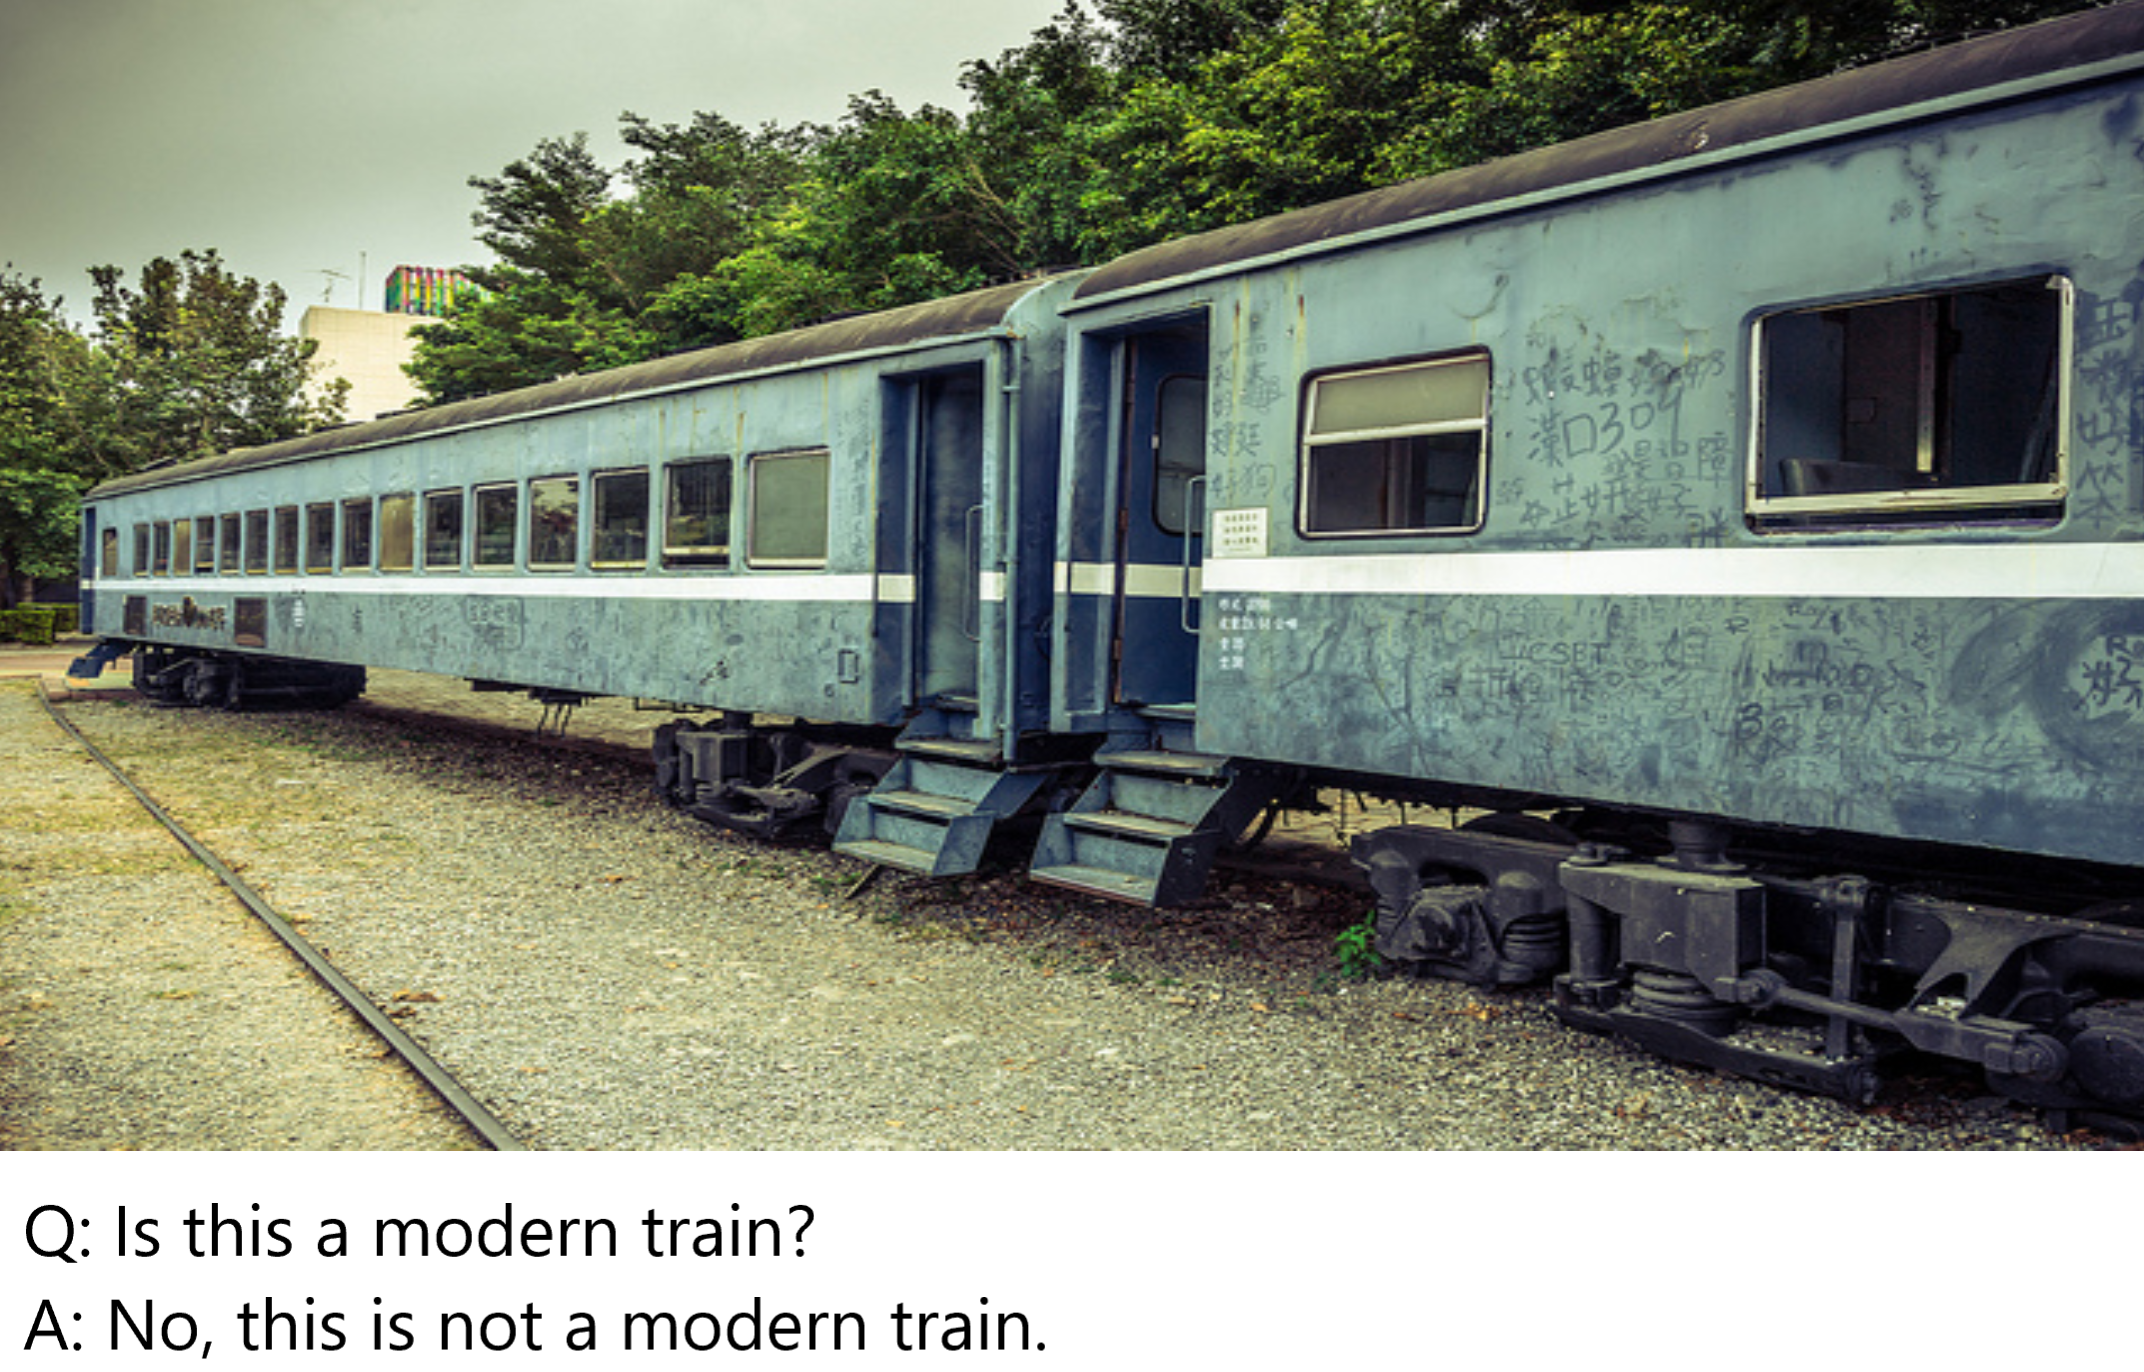
\includegraphics[width=0.7\textwidth]{figs/Intro_objective_train.png}}
    %     \caption{یک نمونه از جفت پرسش‌ و تصویر همراه با پاسخ مورد انتظار}
    %     \label{fig:intro_train}
    % \end{figure}
}
\section{ساختار گزارش}
\paragraph{}
{
    در این پروژه هدف ارائه 
    روشی نو برای حل مسئله کنترل و پایش دستگاه‌های اینترنت اشیاء بر سکوی کوبرنیتز است. 
    در ابتدا به معرفی مفاهیم پایه استفاده شده در این پروژه 
    و سپس به معرفی روش‌ها و کارهای مرتبط پرداخته‌ 
    خواهد شد. پس از آن به معرفی 
    روش و ارزیابی آن پرداخته شده است. در انتها نتیجه‌گیری و 
    کارهای آینده معرفی می‌شوند. 


}